\chapter{Results and analysis}

\section{PSNR SCORE}
The Peak-signal-to-noise ratio (PSNR) score is an engineering term for the ratio between the maximum possible power of a signal and the power of corrupting noise that affects the fidelity of its representation.PSNR score is used for Image super-resolution works as an accuracy measurment even though they can't model human perceptual similarity

PSNR score is easily defined via the mean squared error(MSE).Given the high resolution image $I^{HR}$ and super resolved image $I^{SR}$,MSE is defined as:
\begin{equation}
MSE = \frac{1}{mn}\sum_{i=0}^{m-1}\sum_{j=0}^{n-1}{[I^{SR} - I^{HR}]}^2
\end{equation}
The PSNR (in dB) is defined as:
\begin{equation}
PSNR = 20 log_{10}(MAX_I) - 10 log_{10}(MSE)
\end{equation}
Here, $MAX_i$ is the maximum possible pixel value of the image.In our case $MAX_I = 255$ 

The accuracy of the network where tested against two bechmarks 'Set5' and 'Set14' and the corresponding average psnr score for each of them where calculated and comparing with the trivial bicubic method the SRResNet and SRGAN network performed well in case of psnr score.The SRResNet performed well in reducing the PSNR Score since the generator was only focused on reducing the content loss of the network. The SRGAN network's visual quality was supreme than that of SRResNet even though the PSNR Score was less than that of SRResNet.The SRGAN also had to reduce the adversarial loss of the network which led to an increase in perceptual similarity of the network to that of the original high resolution image.
\begin{center}
\begin{tabular}{|m{3cm} | m{3cm} | m{3cm} |m{3cm}|}
 \hline
 \textbf{Dataset} & \textbf{BICUBIC} & \textbf{SRRESNET} & \textbf{SRGAN}\\
 \hline
 Set5 &28.43&33.096&32.84 \\
\hline
 Set14 &24.64 &31.95 &31.90 \\
 \hline
\end{tabular}
\end{center}
\section{Result Visualization}
The Images from standard benchmark where downsampled using bicubic interpolation and where upscaled using both trained SRResNet Model(consisting only the generator) and SRGAN Model.Some samples of the results are shown in figure: \ref{fig:sampleoutput} 
\begin{figure}[h]
\centering
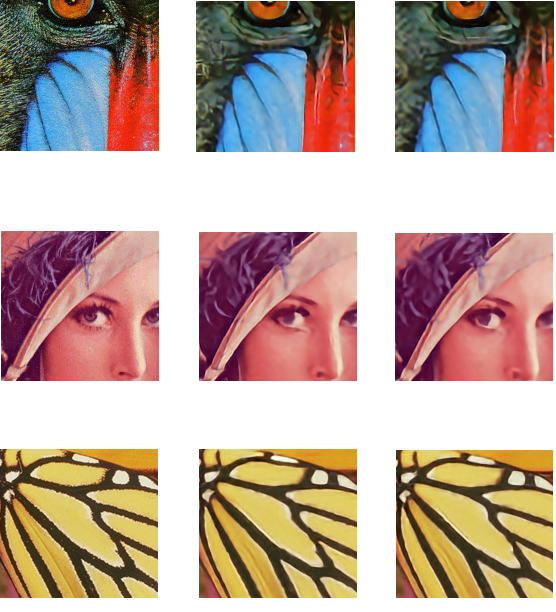
\includegraphics[scale=0.5]{sample_output}
\caption{Comparision of sample Ground Truth Image, SRGAN Image and SRRESNET Image}
\label{fig:sampleoutput}
\end{figure}
From Figure \ref{fig:sampleoutput} it is observed the SRResNet doesn't try to maintain the texture of the high resolution image, instead it reaches the average choice of the high resolution image in the corresponding pixel space.The SRGAN generated image tries to maintain the texture of the image to make them more convincing to the human perceptors.
\subsection{SRResNet}
The figure \ref{fig:srresnetloss} shows the plot of loss against the number of epochs. Where the model where trained using \textbf{NVIDIA QUADRO 5000 GPU}. The training took 48hrs to complete 500 epochs with an initial learning rate of $10^{-4}$ exponentially stepped down every 200 epochs by $10^{-1}$ using DiVerse 2K resolution (DIV2K) dataset containg 291 images and augmenting 85,765 image out of them.
\begin{figure}[h]
\centering
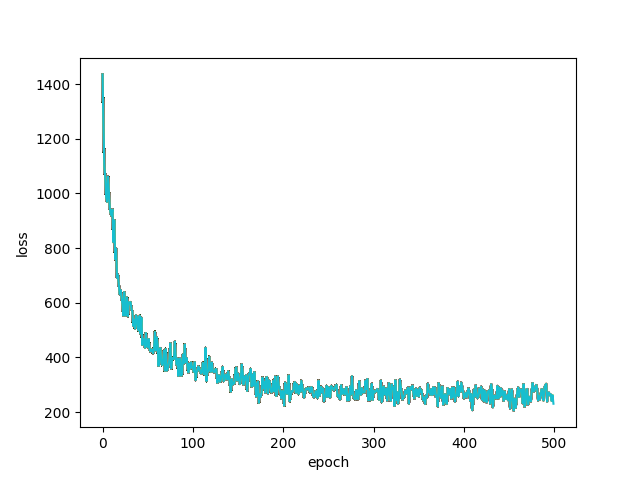
\includegraphics[scale=0.8]{srresnet_loss}
\caption{Plot of loss against number of Epochs for SRResNet}
\label{fig:srresnetloss}
\end{figure}
\subsection{SRGAN}
\begin{figure}[h]
\centering
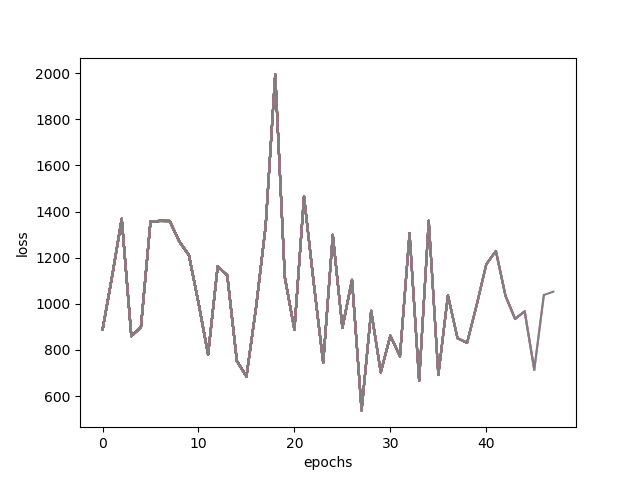
\includegraphics[scale=0.8]{srgan_loss}
\caption{Plot of loss against number of Epochs for SRGAN}
\label{fig:srganloss}
\end{figure}
The figure \ref{fig:srganloss} shows the plot of loss against the number of epochs. Where the model where trained using \textbf{NVIDIA QUADRO 5000 GPU}. The training took 72hrs to complete 500 epochs with both generator and discriminator with an initial learning rate of $10^{-4}$ exponentially stepped down every 200 epochs by $10^{-1}$ using DiVerse 2K resolution (DIV2K) dataset containg 291 images and augmenting 85,765 image out of them..
